\documentclass[sigconf,nonacm]{acmart}

\usepackage{amsmath}
\usepackage{amsfonts}
\let\Bbbk\undefined
\usepackage{amssymb}
\usepackage{booktabs}
\usepackage{multirow}
\usepackage{graphicx}
\usepackage{algorithm}
\usepackage{algorithmic}
\graphicspath{{../results/}{./}}

\settopmatter{printacmref=false}
\setcopyright{none}
\renewcommand\footnotetextcopyrightpermission[1]{}
\pagestyle{plain}

% Math shortcuts
\newcommand{\eps}{\varepsilon}
\newcommand{\E}{\mathbb{E}}
\newcommand{\Prob}{\mathbb{P}}
\newcommand{\Lap}{\mathrm{Lap}}
\DeclareMathOperator{\Var}{Var}
\newtheorem{prop}{Proposition}
\newtheorem{defn}{Definition}

\begin{document}

\title{A Statistical Model of Privacy-Budget Consumption in Repeated Aggregate SQL Workloads}
\subtitle{CMP653 Term Project --- Final Paper}

\author{Refik Can \"Ozta\c{s}}
\affiliation{%
  \institution{Hacettepe University}
  \city{Ankara}
  \country{Turkey}
}
\email{N25142279}

\begin{abstract}
Differentially private (DP) SQL systems answer aggregate queries by adding calibrated noise, but they treat each query in isolation and charge a fresh slice of a finite privacy budget for every release. Real analytical workloads, however, \emph{repeat}: dashboards refresh the same tiles, and drill-downs sweep the same templates. We present a closed-form analytical model that relates a workload's template-repetition structure to its DP privacy-budget consumption. The model's core is the expected distinct-template count $\E[u_k]=\sum_i\bigl[1-(1-p_i)^k\bigr]$; from it we derive the workload-aware budget $\eps_q\E[u_k]$, a savings law $S(k)=1-\E[u_k]/k$ with two limits (deterministic repetition recovers the $1-1/k$ rule; uniform-over-many recovers naive composition), a Zipf-monotonicity result, a variance-aware concentration bound, and a utility ratio $k/\E[u_k]$. We instantiate the model in a unit-tested DP-SQL middleware over DuckDB/PostgreSQL that supports COUNT/SUM/AVG/GROUP BY and top-$k$ (as DP post-processing), and validate it on a $4{,}155$-trial campaign over Zipf workloads, TPC-H (SF=1 and SF=10), and UCI Adult: the model predicts $\E[u_k]$ within $<3\%$ in $21/24$ main-grid cells, is invariant to data scale and to $\eps_q$, and holds \emph{exactly} on a constructed mixed workload. We add two leakage experiments (membership inference and a differencing reconstruction) that confirm the per-query calibration and expose the looseness of cumulative-budget bounds. We are explicit about limits: the validation is a Monte-Carlo self-consistency check, not a real-trace study, and savings vanish on genuinely unique workloads---which the model predicts rather than hides.
\end{abstract}

\maketitle

%% ============================================================
\section{Introduction and Motivation}
\label{sec:intro}

\paragraph{Why this matters.}
Aggregate statistics leak. A pair of COUNT queries that differ by one predicate reveals an individual's attribute by differencing; repeated over a dataset, such queries reconstruct it~\cite{dinur2003revealing}. Differential privacy (DP)~\cite{dwork2006calibrating,dwork2014algorithmic} is the standard defense: perturb each answer with noise calibrated to the query's sensitivity and a per-query budget $\eps_q$, and bound the cumulative privacy loss by composition. The budget is a hard, non-renewable resource: once the total $\sum\eps_q$ reaches a cap $B$, no further query can be answered without breaking the guarantee. A data custodian therefore needs to understand, and ideally predict, \emph{how fast a workload spends its budget}.

\paragraph{A concrete pain.}
Consider an analytics team that publishes a privacy-protected dashboard: a fixed set of tiles (counts, sums, group-by breakdowns) refreshed on a schedule, plus occasional ad-hoc drill-downs. The custodian sets a monthly budget $B$ and a per-query $\eps_q$. Two failures follow from treating queries in isolation. If $\eps_q$ is set to meet an accuracy target, naive composition exhausts $B$ after only $B/\eps_q$ releases and the dashboard goes dark mid-month. If $\eps_q$ is set small enough to survive the month, every tile is needlessly noisy. The custodian cannot tell, in advance, which will happen---because no model relates the \emph{shape} of the workload (how much it repeats) to the budget it will spend. The repetition is exactly the structure our model exploits: the same dashboard tiles recur, so the budget is governed by the handful of \emph{distinct} templates, not the hundreds of refreshes.

\paragraph{The opening: workloads repeat.}
Existing DP-SQL systems (PINQ~\cite{mcsherry2009privacy}, PrivateSQL~\cite{kotsogiannis2019privatesql}, Chorus~\cite{johnson2020chorus}) charge every query a fresh $\eps_q$ and account for them in isolation. Yet analytical workloads are highly repetitive: a monitoring dashboard re-issues the same KPI tile on a schedule, and an analyst's drill-down revisits the same templates with different literals. Under exact-repeat caching, a repeated answer is free (it is \emph{post-processing} of an already-released value), so the budget a workload of length $k$ consumes is governed not by $k$ but by its number of \emph{distinct} queries $u_k$ (Figure~\ref{fig:concept}). The central question of this project is whether $u_k$---and hence the budget---can be \emph{predicted from the workload's repetition structure}, in closed form, before the workload runs.

\begin{figure}[t]
\centering

\includegraphics[width=0.95\columnwidth]{fig_concept}
\caption{Naive composition charges every one of $k$ queries; workload-aware accounting charges only the $u_k$ distinct templates, since repeats are served from cache by post-processing. The model predicts $\E[u_k]$, and hence the budget, before execution.}
\label{fig:concept}
\end{figure}

\paragraph{Contributions.}
\begin{enumerate}
  \item \textbf{An analytical model} (Section~\ref{sec:method}) that, given a template distribution $\{p_i\}$ and length $k$, predicts the expected distinct-query count $\E[u_k]$, the workload-aware budget $\eps_q\E[u_k]$, and the savings ratio $S(k)$, in closed form. Five propositions cover $\E[u_k]$, savings, the Zipf-parameterized case, concentration, and per-query utility, with two named limits that recover the folklore $1-1/k$ rule and naive composition as corners.
  \item \textbf{A middleware} that instantiates the model over DuckDB/PostgreSQL with four execution modes, exact-repeat caching, a temporal (staleness/update) extension, and \textbf{top-$k$ as DP post-processing}.
  \item \textbf{Empirical validation} (Section~\ref{sec:results}) on a $4{,}155$-trial campaign: the model predicts $\E[u_k]$ within $<3\%$ in $21/24$ main-grid cells, is invariant to data scale (SF=1 vs SF=10) and to $\eps_q$, and is exact on a constructed mixed workload; plus two leakage experiments and a runtime analysis.
\end{enumerate}
Throughout, we aim to be balanced and explicit about scope: the headline validation is a self-consistency check (Section~\ref{sec:discussion}), and we report the regimes where the model predicts \emph{no} benefit rather than overclaiming. The predictive allocator that the model also enables, and the learned-allocator comparison, are summarized in Appendix~\ref{app:allocator}; the negative result on semantic caching is in Appendix~\ref{app:semantic}.

%% ============================================================
\section{Related Work}
\label{sec:related}

\paragraph{DP-SQL systems.}
PINQ~\cite{mcsherry2009privacy} introduced composable DP query operators; PrivateSQL~\cite{kotsogiannis2019privatesql} allocates budget across materialized views over a representative workload; Chorus~\cite{johnson2020chorus} rewrites SQL to enforce DP; DOP-SQL~\cite{yu2024dopsql} tunes per-query mechanisms. All expose a \emph{fixed} per-query $\eps_q$ chosen up front and account for queries in isolation; none forecasts a workload's aggregate consumption from its repetition structure.

\paragraph{Workload-aware DP and caching.}
The matrix mechanism~\cite{li2015matrix} optimizes noise for a \emph{known} batch of linear queries, and Dong, Sun, and Yi~\cite{dong2023better} beat worst-case composition by exploiting relational structure. DP caches make repeated work cheaper at runtime: Turbo~\cite{kostopoulou2023turbo} conserves $1.7$--$15.9\times$ budget by generalizing across overlapping linear queries, and CacheDP~\cite{mazmudar2023cachedp} answers a workload at lower budget under an accuracy contract. These deliver the \emph{savings} our model prices, but reactively and without a closed-form forecast; our exact-repeat caching is a simple special case and we claim no novelty for the mechanism itself (Section~\ref{sec:results}).

\paragraph{Multi-query accounting and online allocation.}
Tight composition---moments accountant~\cite{abadi2016deep}, R\'enyi DP~\cite{mironov2017renyi}, zCDP~\cite{bun2016concentrated}---reduces the \emph{rate} of budget spend and is orthogonal to our \emph{count} of distinct releases. APEx~\cite{ge2019apex} translates a per-query accuracy target into the minimum $\eps$ at runtime, one query at a time; BGTplanner~\cite{zhang2024bgtplanner} learns a Gaussian-process-plus-bandit budget policy for federated-learning rounds, driven by an observed-utility signal. Both decide budget reactively, whereas we forecast it from workload structure. A separate line \emph{schedules} a known budget across competing tasks or analysts---privacy budget scheduling and its fairness variants, and multi-analyst budget sharing~\cite{pujol2023multianalyst}, which invokes the coupon-collector problem to bound queries-per-analyst (a throughput limit across \emph{analysts}, not a distinct-template forecast). These take per-task demands as input rather than predicting them.

\paragraph{The model's place.}
Our work sits at the intersection of two mature lines---DP-SQL accounting and unseen-species estimation---neither of which, to our knowledge, has been used to \emph{forecast} a repeated workload's budget. We borrow the occupancy mathematics and the exact-repeat caching mechanism (claiming novelty for neither) and contribute the link: a closed-form, before-execution prediction of $S(k)$ from $\{p_i\}$, with the limit, concentration, and utility consequences that follow.

\paragraph{Distinct counts and unseen species.}
Predicting the number of distinct templates in a length-$k$ workload is the classical unseen-species problem. The occupancy identity $\E[u_k]=\sum_i[1-(1-p_i)^k]$ is textbook~\cite{flajolet1992}; horizon-aware extrapolators---Good--Toulmin~\cite{goodtoulmin1956} and its smoothed variant~\cite{orlitsky2016unseen}---predict new species from a prefix, while richness estimators such as Chao1~\cite{chao1984} estimate total richness. We connect these to DP-budget forecasting; query-template forecasting itself (QueryBot~5000~\cite{ma2018qb5000}) is non-private.

\begin{table}[t]
\footnotesize\centering
\caption{Positioning. No prior system predicts a repeated workload's budget from its structure, before execution.}
\label{tab:related}
\begin{tabular}{l|ccc}
\toprule
System & workload model & predict budget & exact-repeat free \\
\midrule
PINQ/Chorus/PrivateSQL & --- & no & no \\
Turbo / CacheDP        & --- & no & yes (reactive) \\
APEx                   & --- & no (per-query) & no \\
BGTplanner             & learned GP & no & no \\
\textbf{Ours}          & \textbf{closed-form} & \textbf{yes (a-priori)} & \textbf{yes} \\
\bottomrule
\end{tabular}
\end{table}

\paragraph{The gap.}
No prior DP-SQL system gives a closed-form, before-execution prediction of how much budget a \emph{repeated} workload will consume as a function of its template-repetition structure. That prediction---and the limits, concentration, and utility consequences derived from it---is the contribution of this project.

%% ============================================================
\section{Methodology}
\label{sec:method}

\subsection{Threat model and preliminaries}
\label{sec:prelim}

A relational dataset $D$ (DuckDB or PostgreSQL) is queried through the middleware. The adversary is any analyst who can adaptively issue supported queries and observe the noisy outputs; the goal is to bound inference about any single tuple.

\begin{defn}[Tuple-level neighbours]
$D\sim D'$ iff they differ in exactly one tuple (unbounded model).
\end{defn}
\begin{defn}[$\eps$-DP~\cite{dwork2006calibrating}]
$\mathcal{M}$ is $\eps$-DP iff $\Prob[\mathcal{M}(D)\in S]\le e^\eps\,\Prob[\mathcal{M}(D')\in S]$ for every neighbour pair and measurable $S$.
\end{defn}

\paragraph{Supported SQL and sensitivities.}
We support \textsc{select} with COUNT/SUM/AVG, single-table FROM, conjunctive WHERE, and optional GROUP BY. Tuple-level sensitivities are $\Delta f=1$ for COUNT, $\Delta f=B_c$ for SUM($c$) with a per-column clip bound $|c|\le B_c$, and---conservatively---$\Delta f=B_c$ for AVG (a worst-case group of size one, avoiding the implicit $n$-leak of the empirical-mean mechanism, since $n$ is itself private).

\paragraph{Laplace release and composition.}
For sensitivity $\Delta f$ and budget $\eps_q$ the middleware returns $\tilde f(D)=f(D)+\eta$, $\eta\sim\Lap(\Delta f/\eps_q)$. A GROUP BY with $g$ groups noises each group independently; since a tuple affects at most one group, \emph{parallel composition} gives total cost $\eps_q$, not $g\eps_q$. This charges the aggregate \emph{values} only, under the standard DP-histogram assumption that the group-key set is a public categorical domain fixed by the schema (e.g.\ the finite \texttt{education} levels); sensitive or unbounded key domains would require stability-based thresholding and are out of scope. Multi-aggregate queries split $\eps_q$ evenly across aggregates by sequential composition. The exact-repeat cache returns a previously released answer with zero budget cost, since it is post-processing.

\paragraph{Top-$k$ as post-processing.}
The middleware supports top-$k$ (\texttt{$\ldots$ GROUP BY $g$ ORDER BY agg LIMIT $k$}) with one essential design point: ordering and truncation act on the \emph{noised} histogram, never the true one. The engine fetches all $g$ groups, noises every count under the same parallel composition (cost $\eps_q$, \emph{not} $k\eps_q$), and only then sorts by the noisy value and keeps the top $k$. The raw \texttt{ORDER BY/LIMIT} is stripped before it reaches the database---letting the DB apply it would select the reported groups on their \emph{true} counts and leak which groups crossed the cutoff. Because the released slate and its counts are a deterministic function of the $\eps_q$-DP noisy histogram, top-$k$ is post-processing and charges no extra budget (a report-noisy-max guarantee covering the whole top-$k$ list at the cost of one histogram). The price is that selection is \emph{approximate}: groups whose true counts straddle the $k$-th boundary may swap. The forecast and cache apply unchanged---a repeated top-$k$ query is one template, free on exact repeat and counted once in $\E[u_k]$.

\paragraph{Assumptions.}
The forecast assumes (i) a \emph{non-adaptive} analyst whose template choices are independent of the released noise, and (ii) that the template count $m$ and distribution $\{p_i\}$ are public properties of the \emph{query stream}, not of the protected rows. Privacy holds regardless (composition is adaptive-safe and total spend is hard-capped at $B$); the assumptions concern only the average-case \emph{forecast} (Section~\ref{sec:discussion}).

\subsection{The analytical model}
\label{sec:model}

Let $m$ be the number of distinct query templates and $\{p_i\}_{i=1}^m$ a distribution over them; the analyst issues $k$ queries i.i.d.\ from $\{p_i\}$. The cache key is the exact (template, parameter) pair. Let $u_k$ be the number of distinct templates that appear at least once.

\begin{prop}[Expected unique queries]
\label{prop:eu}
$\E[u_k]=\sum_{i=1}^m\bigl[1-(1-p_i)^k\bigr]$.
\end{prop}
\begin{proof}
Let $X_i=\mathbf 1[\text{template }i\text{ appears}]$. Then $\Prob[X_i=0]=(1-p_i)^k$, so $\E[X_i]=1-(1-p_i)^k$; linearity of expectation gives the result.
\end{proof}

\begin{prop}[Budget consumption and savings]
\label{prop:savings}
Naive sequential composition spends $\eps_{\mathrm{naive}}(k)=k\eps_q$. Under workload-aware exact-repeat accounting,
\[
\E[\eps_{\mathrm{wa}}(k)]=\eps_q\,\E[u_k],\qquad
S(k)=1-\frac{\E[\eps_{\mathrm{wa}}(k)]}{\eps_{\mathrm{naive}}(k)}=1-\frac{1}{k}\sum_i\bigl[1-(1-p_i)^k\bigr].
\]
\end{prop}

\noindent\textbf{Limits.} \emph{(A) Deterministic repetition} ($p_1{=}1$): $S(k)=1-1/k$---the folklore rule, now a corner of Proposition~\ref{prop:savings} at maximum skew, not a standalone claim. \emph{(B) Uniform, $m\to\infty$}: workloads almost never repeat, $\E[u_k]\to k$, $S(k)\to0$, recovering naive composition. \emph{(C) Uniform, $k\to\infty$, $m$ fixed}: every template eventually appears, so the budget saturates at $m\eps_q$ regardless of $k$---the practical regime in which a finite-template workload cannot exhaust a budget large enough to cover all $m$ templates.

\begin{prop}[Zipf-parameterized workload]
\label{prop:zipf}
For $p_i\propto i^{-\alpha}$, the savings ratio $S(k)$ is monotone non-decreasing in $\alpha$ for fixed $(k,m)$, approaching Limit~B as $\alpha\to0$ and Limit~A as $\alpha\to\infty$.
\end{prop}
\begin{proof}[Proof sketch]
$\E[u_k]=\sum_i\phi(p_i)$ with $\phi(x)=1-(1-x)^k$ concave ($\phi''\le0$), so $\E[u_k]$ is Schur-concave. Larger $\alpha$ majorizes the weight vector (mass shifts onto top templates), hence lowers $\E[u_k]$ and raises $S(k)$; the endpoints follow from the uniform and point-mass cases. A numerical scan over $m\in\{3,\dots,100\}$, $k\in\{2,\dots,200\}$ found no violation.
\end{proof}

\begin{prop}[Concentration of $u_k$]
\label{prop:conc}
Writing $u_k=\sum_iX_i$ with $q_i=1-(1-p_i)^k$, the occupancy indicators are negatively associated, so
$\Var[u_k]\le\sum_i q_i(1-q_i)\le m/4=:V$, and Chebyshev gives $\Prob[|u_k-\E[u_k]|\ge t]\le V/t^2$.
\end{prop}

\noindent Because $V=O(m)$ rather than $O(k)$, the realized $u_k$ has standard deviation $\sqrt V=O(\sqrt m)$, so a \emph{single} workload lands within a fraction of a template of the forecast (a distribution-free McDiarmid bound $2e^{-2t^2/k}$ also holds but is $\sim18\times$ looser once $u_k$ saturates and we report it only as a fallback). The budget-exhaustion tail follows: for $c/\eps_q>\E[u_k]$, $\Prob[u_k\eps_q\ge c]\le V/(c/\eps_q-\E[u_k])^2$.

\begin{prop}[Utility under a fixed total budget]
\label{prop:util}
With a fixed total $\eps_{\mathrm{tot}}$, naive affords $\eps_q^{\mathrm{naive}}=\eps_{\mathrm{tot}}/k$ per query and workload-aware affords $\eps_q^{\mathrm{wa}}=\eps_{\mathrm{tot}}/\E[u_k]$ per unique release; since $\E[|\eta|]=\Delta f/\eps_q$, the predicted per-query error ratio is $k/\E[u_k]$.
\end{prop}

\noindent At Zipf $\alpha{=}1$, $m{=}10$, $k{=}100$, $\E[u_k]\approx9.9$, so workload-aware accounting answers the same workload at roughly $10\times$ lower per-query error at equal total budget. One honest caveat: a cached answer reuses a \emph{single} noise draw, forgoing the variance reduction of $k$ independent draws---the budget saving and the lost averaging are two sides of the same coin.

\subsection{System and temporal extension}
\label{sec:system}

The middleware is a thin proxy between the analyst and a backend database (Figure~\ref{fig:arch}). Each query is parsed and validated, hashed to a (template, parameter) key, and checked against a two-level cache; a hit is returned for free (post-processing), a miss is charged $\eps_q$, noised, and cached. Four execution modes (exact, naive-DP, workload-aware-DP, temporal-DP) share the pipeline of Algorithm~\ref{alg:full}, which couples cache validity to a temporal regime: it advances a logical clock, simulates Poisson-rate invalidations, ages each entry against the staleness tolerance $\tau$, and only then returns the cached release or charges the ledger.

\begin{figure}[t]
\centering
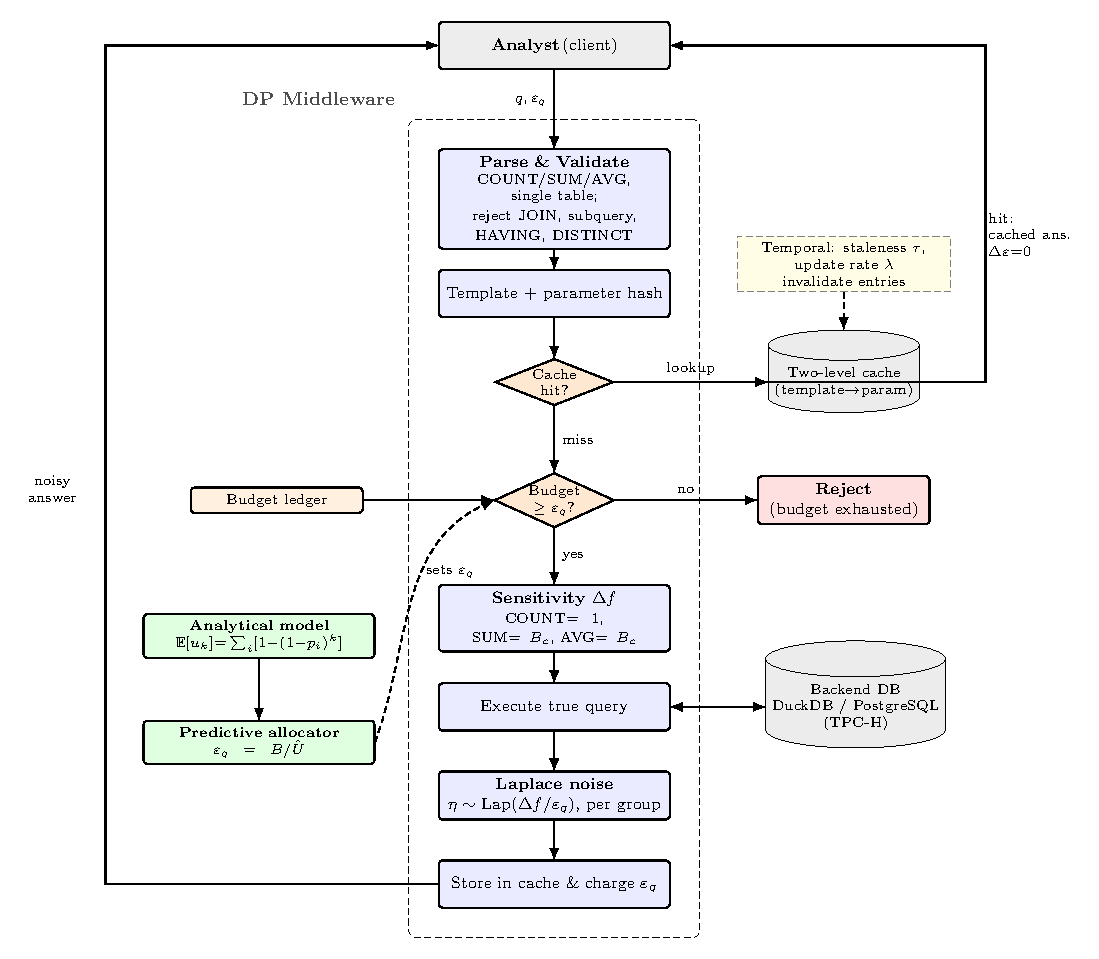
\includegraphics[width=0.86\columnwidth]{fig_arch}
\caption{Workload-aware DP-SQL middleware. A cache hit is free by post-processing; a miss is charged $\eps_q$, noised, and cached. The analytical model drives the predictive allocator ($\eps_q{=}B/\hat U$), and a temporal regime $(\tau,\lambda)$ invalidates stale entries.}
\label{fig:arch}
\end{figure}

\begin{algorithm}[t]
\caption{Workload-aware DP middleware (one query).}
\label{alg:full}
\begin{algorithmic}[1]
\REQUIRE Query $q$, budget $\eps_q$, ledger $\mathcal L$, staleness $\tau$, update $(\lambda,q_{\mathrm{inv}})$
\STATE Parse/validate $q$; advance clock; invalidate each entry w.p.\ $\lambda q_{\mathrm{inv}}$
\STATE Compute template hash $h_T$, parameter hash $h_P$
\IF{$\mathcal L.\mathrm{cache}[h_T][h_P]$ fresh (age $\le\tau$)}
   \STATE \textbf{return} cached $\tilde r$ \hfill {\small (post-processing, $\Delta\eps{=}0$)}
\ENDIF
\IF{$\mathcal L.\mathrm{remaining}<\eps_q$} \STATE \textbf{return} \textsc{BudgetExhausted} \ENDIF
\STATE $\Delta f\gets$ sensitivity; $\mathcal L.\mathrm{consumed}\mathrel{+}=\eps_q$
\STATE $r\gets$ execute $q$; $\tilde r\gets r+\Lap(\Delta f/\eps_q)$ per aggregate, per group
\STATE Cache and \textbf{return} $\tilde r$
\end{algorithmic}
\end{algorithm}

A \emph{temporal extension} couples budget to time, addressing the milestone note that ``budget and temporality should be considered together'': data updates invalidate cached answers and freshness requirements force re-noising.

\begin{prop}[Temporal budget]
\label{prop:temporal}
With horizon $T$, staleness tolerance $\tau$, update rate $\lambda$, and per-update invalidation probability $q$, the expected number of (re-)noisings per template is $N=\max(1,\lceil T/\tau\rceil)+T\lambda q$, so $\E[\eps_{\mathrm{temp}}]=\eps_q\,\E[u_k]\,N$.
\end{prop}

\noindent Three regimes are continuous slidings of one expression: \emph{(a) static snapshot} ($\tau\to\infty,\lambda{=}0,N{=}1$) recovers Section~\ref{sec:model}; \emph{(b) bounded staleness} ($\tau$ finite, $\lambda{=}0$, $N{=}\lceil T/\tau\rceil$); \emph{(c) update-driven} ($\lambda{>}0$, $N$ grows linearly in $T$). The prototype is unit-tested across parser validation, sensitivity, Laplace calibration, cache semantics, the model limits, the concentration bound, and temporal re-noising.

%% ============================================================
\section{Results and Findings}
\label{sec:results}

\paragraph{Setup.}
The campaign comprises \textbf{six sweeps totaling $4{,}155$ trials} ($\sim$$150{,}000$ queries) over Zipf workloads ($m{=}7$ Adult age-bands and TPC-H templates), four per-query budgets $\eps_q\in\{0.1,0.5,1,2\}$, lengths $k\in\{10,\dots,500\}$, and two data scales (TPC-H SF=1 with 6M lineitem rows, SF=10 with 60M). Comparisons are between internal execution modes under an identical middleware, to isolate the algorithmic effect of workload-aware accounting; end-to-end comparison against external prototypes would require query-rewriting integration and is left as future work.

\subsection{Validating the model}

\paragraph{Model vs.\ empirical $\E[u_k]$.}
Table~\ref{tab:validation} compares the closed form to the 30-trial empirical mean across the main grid: agreement is within $<3\%$ in \textbf{$21$ of $24$ cells}; the three outliers ($3.5$--$8.6\%$) occur at high skew and small $k$, where $\E[u_k]$ is tiny and a $0.1$-unit deviation is a large relative error. The savings ratio $S(k)$, computed from measured budget, matches within $<2\%$ in $23/24$ cells.

\begin{table}[t]
\caption{Model vs.\ empirical $u_k$, Zipf ($m{=}7$, 30 trials/cell). Parentheses: signed relative error (\%).}
\label{tab:validation}
\centering\small
\begin{tabular}{c|cccc}
\toprule
$\alpha\backslash k$ & 10 & 25 & 50 & 100 \\
\midrule
0.0 & 5.50/5.53 ($-0.6$) & 6.85/6.77 ($1.2$) & 7.00/7.00 ($0.0$) & 7.00/7.00 ($0.0$) \\
0.5 & 5.30/5.23 ($1.3$) & 6.73/6.73 ($-0.1$) & 6.98/6.93 ($0.7$) & 7.00/7.00 ($0.0$) \\
1.0 & 4.73/4.70 ($0.6$) & 6.32/6.30 ($0.3$) & 6.88/6.90 ($-0.3$) & 7.00/7.00 ($0.0$) \\
1.5 & 3.98/3.87 ($2.8$) & 5.57/5.70 ($-2.3$) & 6.48/6.40 ($1.3$) & 6.91/6.93 ($-0.3$) \\
2.0 & 3.25/3.13 ($3.5$) & 4.64/4.70 ($-1.3$) & 5.69/5.73 ($-0.7$) & 6.50/6.43 ($1.1$) \\
3.0 & 2.19/2.07 ($5.7$) & 3.07/3.33 ($-8.6$) & 3.85/3.90 ($-1.3$) & 4.72/4.67 ($1.1$) \\
\bottomrule
\end{tabular}
\end{table}

\paragraph{Invariance and limits.}
The model's $\E[u_k]$ is structurally independent of $\eps_q$ (confirmed within $0.12$ units across $\eps_q\in\{0.1,0.5,1,2\}$) and of data scale: the same templates over a $10\times$ larger TPC-H database (60M rows) give identical empirical $\E[u_k]$ to within $0.034$ units, isolating workload structure from data scale. Pushing skew to $\alpha{=}10$ at $k{=}200$, predicted and empirical $\E[u_k]$ stay within $0.13$ units while $\E[u_k]$ varies by an order of magnitude, and $S(k)\to99.4\%$ recovers the $1-1/k$ corner numerically (Figure~\ref{fig:limits}).

\begin{figure}[h]
\centering

\includegraphics[width=0.92\columnwidth]{model_validation/model_validation_limits.png}
\caption{Savings ratio $S(k)$ vs.\ workload length, several Zipf $\alpha$. Dashed: model. Markers: empirical mean (30 trials). High-$\alpha$ curves approach $1-1/k$ (Limit~A); the $\alpha{=}0$ curve stays near $0$ until $k$ approaches $m$ (Limit~B).}
\label{fig:limits}
\end{figure}

\paragraph{Robustness.}
Four properties make the forecast dependable. \emph{(i) Distribution-agnostic}: it is exact for any i.i.d.\ marginal (uniform, Zipf, lognormal-shaped), matching the empirical mean to $\le0.2$. \emph{(ii) Concentrated}: by Proposition~\ref{prop:conc}, $\sqrt V{=}0.34$--$1.22$ at $m{=}20$, so a single run is reliable, not merely the expectation. \emph{(iii) Exact on heterogeneous workloads}: on a constructed mixed W1+W4 workload with true $u_k=1+(1-f)k$, the closed form $\eps_q u_k$ matches the measured budget \emph{to the cent} at every mixing fraction (Table~\ref{tab:mixed}). \emph{(iv) Conservative under correlation}: a bursty sticky-Markov process (same stationary marginal) lowers the distinct count, so the i.i.d.\ forecast \emph{over}-predicts $u_k$ by $1.09$/$1.29$/$2.72\times$ at stickiness $s{=}0.3$/$0.6$/$0.9$---the safe direction, since $\eps_q\E[u_k]$ then only loosens as an upper bound and the privacy guarantee is never violated. The worst case of this guarantee is the $\eps_q{=}B/m$ allocator: since $u_k\le m$ for \emph{any} arrival process, it never rejects.

\begin{table}[h]
\caption{Mixed W1+W4 workload, $B{=}50$, $\eps_q{=}0.5$, 20 trials. The closed form matches the measured budget exactly.}
\label{tab:mixed}
\centering\small
\begin{tabular}{c|c|cc}
\toprule
$f$ & true $u_k$ & measured $\eps$ used & predicted $\eps_q u_k$ \\
\midrule
0.1 & 91 & 45.5 & 45.5 \\
0.3 & 71 & 35.5 & 35.5 \\
0.5 & 51 & 25.5 & 25.5 \\
0.7 & 31 & 15.5 & 15.5 \\
0.9 & 11 & 5.5  & 5.5  \\
\bottomrule
\end{tabular}
\end{table}

\paragraph{Temporal extension.}
The temporal model is validated by sweeping $\tau$ (with $\lambda{=}0$) and $\lambda$ (with $\tau$ large): the prediction $\E[\eps_{\mathrm{temp}}]=\eps_q\E[u_k]N$ tracks the empirical mean in trend and matches closely at large $\tau$ (rare re-noising), while at small $\tau$ it is a conservative \emph{upper} bound (e.g.\ at $\tau{=}10$ it predicts $\E[\eps]\approx70$ vs.\ an empirical $\approx39$, since not all re-noisings materialize within the horizon). Freshness thus has an explicit, bounded cost.

\subsection{Real-workload validation (Redbench)}
\label{sec:redbench}

The synthetic sweep cannot establish \emph{external} validity, so we add the first test on production-derived traces: Redbench~\cite{redbench2025}, 30 analytical SQL workloads synthesized from Amazon Redshift's Redset query log, in which each user's real query timeline (and thus its repetition structure) is mapped onto CEB+/JOB query instances. The exact-query identity is the SQL instance, so the realized distinct count $u_k$ and Redbench's own \emph{query-repetition rate} $=1-u_k/k$ are exactly our $S(k)$. Running the occupancy model against all 30 workloads (\texttt{experiments/redbench\_validation.py}) yields four findings.
\emph{(1) Real workloads span the full skew range:} realized $S(k)$ runs from $0\%$ to $98\%$ (mean $53\%$), so template repetition---the structure the model exploits---is pervasive in production, not an artefact of the sweep.
\emph{(2) Real distributions are heavy-tailed:} fitting Zipf to each workload gives $\alpha\in[0,3]$ with mean $0.84$ (near classic Zipf), and our synthetic sweep $\alpha\in\{0,\dots,3\}$ \emph{brackets} the real range---answering ``why Zipf?'' with production data.
\emph{(3) The closed form tracks realized savings} to within a mean absolute $0.13$ in $S(k)$, tightest in the high-repetition regime where savings are largest (e.g.\ $0.92$ vs.\ $0.93$, $0.97$ vs.\ $0.98$).
\emph{(4) Forecasting from a $50\%$ prefix}, the smoothed Good--Toulmin estimator~\cite{orlitsky2016unseen} halves the plug-in's error ($0.12$ vs.\ $0.22$ in $u_k/k$), confirming on real data that unseen-species correction is the right tool for prefix-based forecasting. Honestly, Redbench is trace-\emph{derived} synthesis---its repetition structure is real but its queries are CEB+/JOB instances, not raw production SQL---so this raises external validity substantially without fully eliminating it (Section~\ref{sec:discussion}).

\subsection{Budget savings and where naive composition fails}

\paragraph{Full grid.}
Across six workloads, workload-aware accounting answers the same $100$ queries at comparable per-query MAE while spending only $\eps_q u_k$: savings of $100\times$ on the repetitive W1, $33\times$/$20\times$/$14.3\times$ on the TPC-H/uniform pools (where $u_k$ saturates at the pool size $m$), and \emph{exactly} $1\times$ on the genuine drill-down W4, where every query is unique and the model correctly predicts $S(k){=}0$ (Figure~\ref{fig:savings}). These multipliers are accounting ratios $1/(1-S(k))$ that any exact-repeat cache attains; our contribution is the closed-form \emph{prediction} of $S(k)$ before execution (within $<3\%$), not the saving itself.

\begin{table}[h]
\footnotesize\centering
\caption{Full grid (6 workloads, $k{=}100$, $\eps_q{=}1$, 30 trials). Workload-aware spends $\eps_q u_k$ at $93$--$99\%$ cache-hit rates; the drill-down (W4) is the predicted no-win case.}
\label{tab:fullgrid}
\begin{tabular}{l|cc|c}
\toprule
Workload & naive $\eps$ & work.-aware $\eps$ & savings \\
\midrule
W1 Repetitive            & 100.0 & 1.0   & $100\times$ \\
W2 TPC-H returnflag      & 100.0 & 3.0   & $33\times$ \\
W2 TPC-H priority        & 100.0 & 5.0   & $20\times$ \\
W2 Zipf $\alpha{=}1$     & 100.0 & 7.0   & $14.3\times$ \\
W3 Uniform               & 100.0 & 7.0   & $14.3\times$ \\
W4 Drill-down (unique)   & 100.0 & 100.0 & $1\times$ \\
\bottomrule
\end{tabular}
\end{table}

\begin{figure}[h]
\centering
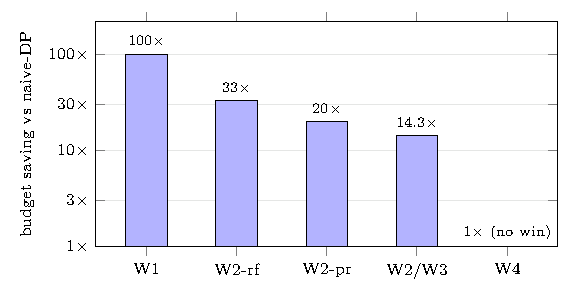
\includegraphics[width=0.92\columnwidth]{fig_savings}
\caption{Budget saved vs.\ naive ($k{=}100$, $\eps_q{=}1$, log scale): up to $100\times$ on the repetitive W1 and $14$--$33\times$ on the parametric/uniform pools, but exactly $1\times$ (no win) on the unique drill-down W4---the model predicts the $S(k){=}0$ case rather than overclaiming.}
\label{fig:savings}
\end{figure}

\paragraph{Real-system baseline.}
To confirm these savings against a \emph{deployed} engine rather than our own naive mode, we run the same workloads through OpenDP SmartNoise-SQL~\cite{smartnoise} (\texttt{experiments/realsystem\_baseline.py}). SmartNoise charges every query against its odometer and has no exact-repeat caching, so on the repetitive dashboard ($k{=}100$ identical COUNT releases at $\eps_q{=}1$) it spends the full $\eps{=}100.0$ where workload-aware accounting spends $1.0$ ($u_k{=}1$; the $99$ repeats are free)---a $100\times$ gap, now against a real library, not an internal baseline. On a genuinely all-distinct workload both spend $100.0$: we \emph{tie}, since there is no repetition to exploit. Both use basic pure-$\eps$ composition here; SmartNoise's tighter R\'enyi accounting would lower \emph{both} rates and is orthogonal to (composes with) the caching---consistent with the model treating tight composition as a separate axis.

\paragraph{Two concrete failure regimes of naive composition.}
On the real middleware (Adult, $B{=}10$, $k{=}100$, 12 trials; Table~\ref{tab:killer}), repetition turns the structural advantage into a stark gap. \emph{(A) Budget exhaustion}: a dashboard re-issuing one tile at fixed $\eps_q{=}1$ exhausts naive after $B/\eps_q{=}10$ queries ($10/100$ answered), while caching answers all $100/100$ for free---a $10\times$ gap. \emph{(B) Accuracy at fixed total budget}: to answer all $100$, naive must thin the budget ($\eps_q{=}B/k{=}0.1$, error $\approx10$), whereas concentrating it on the $u_k{=}1$ distinct release makes the answer essentially exact. \emph{(C, honest counter)}: on a genuine drill-down both match at error $\approx9.6$---included precisely because the model predicts the no-win case.

\begin{table}[h]
\footnotesize\centering
\caption{Naive's failure regimes vs.\ workload-aware (real middleware, Adult, $B{=}10$, $k{=}100$).}
\label{tab:killer}
\begin{tabular}{l|cc|cc}
\toprule
& \multicolumn{2}{c|}{Naive} & \multicolumn{2}{c}{Workload-aware} \\
Workload & ans. & $|$err$|$ & ans. & $|$err$|$ \\
\midrule
Repetitive, fixed $\eps_q{=}1$ & $10/100$ & $0.9$ & $\mathbf{100/100}$ & $0.4$ \\
Repetitive, fixed budget $B$ & $100/100$ & $10.0$ & $100/100$ & $\mathbf{\approx0}$ \\
Drill-down (all unique) & $100/100$ & $9.6$ & $100/100$ & $9.6$ \\
\bottomrule
\end{tabular}
\end{table}

\subsection{Putting the model to work: predictive allocation}

The model is descriptive (it predicts budget from a workload) and also \emph{prescriptive}: an allocator can estimate $\hat U=\E[u_k]$ online from the empirical template distribution (after a short warmup) and set $\eps_q=B/\hat U$ to target the offline optimum $\eps_q^*=B/u_k$ (Proposition~\ref{prop:savings}), capping spend at $B$. At a fixed \emph{total} budget this trades coverage for accuracy: on Zipf workloads ($k{=}100$, $B{=}10$) it cuts per-query MAE versus naive (Table~\ref{tab:predictive}), by point estimates of $16.8\%$ at $\alpha{=}0$ down to $5.4\%$ at $\alpha{=}2$. We are deliberately careful: a paired $t$-test finds the gain significant only at low skew ($p\approx0.05$ at $\alpha{=}0$; $p>0.3$ for $\alpha\ge1$), so it is a low-skew effect, not a uniform win, and it costs some late-query rejections. The robust, regime-independent result is instead the \emph{safe} allocator $\eps_q{=}B/m$, which never rejects ($u_k\le m$) and matches the best operating point of a learned bandit at zero exploration cost (Appendix~\ref{app:allocator}). The MAE reduction is largest in the tightest-budget regime, where every release matters: sweeping $B\in\{1,5,10,50\}$ at $\alpha{=}1$, the predictive allocator cuts MAE by $32\%$ at $B{=}1$ (predictive $68.7$ vs.\ naive $101.1$) and $21\%$ at $B{=}50$. The advantage is structural, not data-dependent: at TPC-H SF=10 (60M rows) it still cuts MAE to $6.03$ vs.\ naive's $10.01$ ($40\%$).

\begin{table}[h]
\footnotesize\centering
\caption{Predictive allocator vs.\ fixed-$\eps_q$ baselines (mean$\pm$SE, 30 trials, $k{=}100$, $B{=}10$). The gain over naive is significant only at $\alpha{=}0$.}
\label{tab:predictive}
\begin{tabular}{c|l|ccc}
\toprule
$\alpha$ & Mode & MAE & answered & $\eps$ spent \\
\midrule
\multirow{2}{*}{0.0} & Naive & 9.86 & 100/100 & 10.0 \\
 & \textbf{Predictive} & \textbf{8.21}$\pm$0.85 & 69/100 & 10.0 \\
\midrule
\multirow{2}{*}{1.0} & Naive & 9.81 & 100/100 & 10.0 \\
 & \textbf{Predictive} & \textbf{8.98}$\pm$0.93 & 78/100 & 10.0 \\
\midrule
\multirow{2}{*}{2.0} & Naive & 9.96 & 100/100 & 10.0 \\
 & \textbf{Predictive} & \textbf{9.42}$\pm$1.40 & 88/100 & 10.0 \\
\bottomrule
\end{tabular}
\end{table}

\subsection{Privacy leakage}

We complement the budget/utility analysis with two attacks that confirm the per-query calibration. \emph{Membership inference}: an adversary observing one noisy COUNT must decide whether a target is present. Empirical AUC tracks the DP upper bound $e^\eps/(1+e^\eps)$ within $\le1\%$ and is no better than chance at $\eps\le0.1$ (Table~\ref{tab:leak}, left). \emph{Reconstruction}: replaying a 5-level differencing drill-down on real Adult counts $(48842,34327,24137,7210,3137)$, the mean absolute error scales as $1.5/\eps$ (the expected difference of two $\Lap(1/\eps)$ variables) to within a few percent across three orders of magnitude (Table~\ref{tab:leak}, right). A stronger shadow-model MIA across four workloads $\times$ four $\eps_q$ (32 cells, 60 shadow runs each) yields AUC $0.14$--$0.58$, far below the cumulative-budget bound's $\to1.0$: \emph{cumulative-budget bounds are loose for realistic workload MIA}, and the per-query $\eps_q$, not the cumulative budget, governs the signal. Both attacks degrade exactly where the model predicts efficient budgeting (high skew, low $\eps_q$), and both succeed on the W4 drill-down---which the model also flags as the no-savings case.

\begin{table}[h]
\footnotesize\centering
\caption{Single-release leakage. Left: membership-inference AUC vs.\ the DP bound. Right: differencing reconstruction error vs.\ the $1.5/\eps$ reference.}
\label{tab:leak}
\begin{tabular}{c|cc||c|cc}
\toprule
$\eps$ & AUC & $\frac{e^\eps}{1+e^\eps}$ & $\eps$ & rec.\ err & $1.5/\eps$ \\
\midrule
0.01 & 0.499 & 0.503 & 0.01 & 148.2 & 150.0 \\
0.10 & 0.522 & 0.525 & 0.10 & 14.8  & 15.0 \\
1.00 & 0.724 & 0.731 & 1.00 & 1.5   & 1.5 \\
5.00 & 0.988 & 0.993 & 5.00 & 0.3   & 0.3 \\
\bottomrule
\end{tabular}
\end{table}

\begin{figure}[h]
\centering
\includegraphics[width=0.92\columnwidth]{workload_leakage/workload_mia_auc.png}
\caption{Shadow-model MIA AUC across W1--W4 at $\eps_q\in\{0.1,0.5,1,2\}$ (32 cells, 60 shadow runs each). Even a classifier seeing the full $k{=}50$ sequence stays far below the cumulative-budget bound ($\to1.0$); most queries do not directly probe the target tuple.}
\label{fig:mia}
\end{figure}

\subsection{Runtime and overhead}

The privacy machinery is cheap relative to I/O. Instrumenting $1{,}500$ queries, cache hits are $2.7\times$ faster than misses ($0.76$ vs.\ $2.02$ ms) because they skip the database round-trip (36\% of miss cost); SQL parsing is 21\%, and the privacy-specific stages (sensitivity, allocation, noise) sum to under $0.25$ ms. Tail latency is controlled (miss $p99{=}5.1$ ms, hit $p99{=}3.6$ ms), and single-threaded throughput is $\sim$$495$ q/s on the miss path and $\sim$$1{,}320$ q/s on the hit path, so a workload-aware mode at $93$--$99\%$ hit rate sustains analyst-tier load. The asymptotic cost of the forecast itself is $O(m)$ per evaluation of $\E[u_k]$.

%% ============================================================
\section{Future Work}
\label{sec:future}
Several extensions follow directly. \emph{(1) Raw production traces:} the Redbench validation uses trace-derived synthesis; running the model on raw analyst query logs (and executing them through a DP engine end-to-end) would close the remaining external-validity gap. \emph{(2) Tight composition:} replacing basic sequential composition with R\'enyi DP~\cite{mironov2017renyi} or zCDP~\cite{bun2016concentrated} would predict $\sum\eps_i$ rather than count $u_k$, with the closed-form structure mostly unchanged---and composes with the caching, as the SmartNoise comparison shows. \emph{(3) Multi-table / JOINs:} the occupancy framework generalizes to JOIN-shaped queries given a per-template sensitivity bound such as residual sensitivity~\cite{dong2021residual} or R2T~\cite{dong2022r2t}. \emph{(4) Equivalence-checked semantic cache:} pairing tree-kernel/embedding similarity with a symbolic equivalence prover (predicate normalization, range merging, $\alpha$-conversion) would let the cache safely admit non-identical-but-equivalent queries (Appendix~\ref{app:semantic}). \emph{(5) Cache re-release and AVG decomposition:} re-noising stale cache entries on budget surplus, and a SUM$+$COUNT decomposition of AVG with per-group accounting, would tighten utility. \emph{(6) Private group-key domains:} a stability-based threshold that suppresses low-count groups would lift the public-key-domain assumption at a small $\delta$ cost.

\section{Discussion and Conclusion}
\label{sec:discussion}

\paragraph{Findings.}
(1) Budget consumption is a function of $\E[u_k]$, not of the cache implementation: $\E[\eps_{\mathrm{wa}}]=\eps_q\E[u_k]$ holds within $<3\%$ in $21/24$ cells, exactly on the mixed workload, and is invariant to scale and $\eps_q$---so a deployment can estimate its privacy cost \emph{before} running a query. (2) The $1-1/k$ rule is the high-skew corner of one model. (3) Cumulative-$\eps$ bounds are loose for realistic MIA (AUC $0.14$--$0.58$). (4) The model is honest about failure: on uniform workloads and drill-downs, savings vanish and reconstruction succeeds, exactly as predicted.

\paragraph{Practical implication.}
Because $\E[u_k]$ is computable before any query runs and is invariant to data scale and $\eps_q$, the custodian of the dashboard scenario can size $\eps_q$ \emph{a priori}: the safe choice $\eps_q=B/m$ provably finishes the month (since $u_k\le m$), and the predictive allocator pushes accuracy further when the workload is skewed. The model also tells the custodian when caching cannot help---a drill-down workload spends like naive composition---so the privacy/utility budget can be planned, not discovered after exhaustion. The same forecast bounds the leakage analysis: budgeting and attack-resistance improve together in the high-skew, low-$\eps_q$ regime.

\paragraph{Threats to validity.}
We separate three. \emph{Construct}: the headline ``$\E[u_k]$ within $<3\%$'' is a Monte-Carlo \emph{self-consistency} check---the empirical $u_k$ is sampled from the very Zipf distribution the closed form integrates, so the mean converges to $\E[u_k]$ \emph{by construction}; it validates the estimator's arithmetic, not the claim that real workloads are i.i.d.\ Zipf. \emph{Internal}: the forecast assumes a non-adaptive analyst; against a worst-case adaptive analyst the only valid bound is $u_k\le\min(k,m)$, i.e.\ the $\eps_q{=}B/m$ safe allocator. \emph{External}: the headline grid is synthetic, but we now validate on Redbench (Section~\ref{sec:redbench})---30 production-\emph{derived} traces spanning $0$--$98\%$ repetition with fitted Zipf $\alpha\in[0,3]$ (mean $0.84$)---which raises external validity substantially. The residual gap is honest: Redbench is trace-\emph{derived} synthesis (real repetition structure, benchmark queries rather than raw production SQL), and the i.i.d.\ closed form is mildly over-optimistic about savings at the low-repetition end. Scope is single-table aggregates under basic composition; JOINs and tight (R\'enyi/zCDP) composition are future work.

\paragraph{Conclusion and reproducibility.}
A closed-form model parameterized by $(\{p_i\},k)$ predicts realized DP-budget consumption in repeated aggregate SQL workloads, recovers the folklore $1-1/k$ rule as a corner, and is validated to $<3\%$ across $4{,}155$ trials---while being explicit about the regimes in which it predicts no benefit. The middleware, all experiment generators, and the canonical result CSVs are public\footnote{\url{https://github.com/canoztas/cmp653-project}} with fixed seeds; the model-validation and allocation experiments are bit-reproducible and the large campaign is distributionally reproducible. The Redbench and SmartNoise-SQL baselines are reproduced by \texttt{experiments/redbench\_validation.py} and \texttt{experiments/realsystem\_baseline.py}.

\appendix

%% ============================================================
\section{Predictive Budget Allocator}
\label{app:allocator}

The model is also \emph{prescriptive}: instead of fixing $\eps_q$ offline, an allocator can estimate $\hat U=\E[u_{k}]$ online from the empirical (Laplace-smoothed) template distribution after a short warmup and set $\eps_q=B/\max(\hat U,1)$, capped to the remaining budget so total spend never exceeds $B$. This targets the offline optimum $\eps_q^*=B/u_k$ (Proposition~\ref{prop:savings}). On Zipf workloads ($k{=}100$, $B{=}10$, 30 trials) the predictive allocator cuts per-query MAE by up to $\sim$$17\%$ at low skew (point estimates $16.8\%$ at $\alpha{=}0$ down to $5.4\%$ at $\alpha{=}2$, and up to $32\%$ in the tightest-budget regime $B{=}1$), but the gain is statistically significant only at low skew (paired $t$-test $p\approx0.05$ at $\alpha{=}0$, $p>0.3$ for $\alpha\ge1$); we report it as a low-skew effect, not a uniform win. The regime-independent result is instead the \emph{safe} allocator $\eps_q{=}B/m$: since $u_k\le m$, it never rejects and needs no warmup, and on the benchmark it answers all queries at fresh-release MAE $2.0$ versus an $\eps$-greedy bandit's $3.8$ at the same $100\%$ rate---a $1.9\times$ gap that is the bandit's exploration tax, since $B/m$ \emph{is} the bandit's best-arm operating point (holding when $m\le k/4$).

\begin{table}[h]
\footnotesize\centering
\caption{Online allocation policies (Zipf, $m{=}20$, $k{=}100$, $B{=}10$, 60 trials). Fresh MAE (over cache misses) is reported jointly with the answered fraction.}
\label{tab:allocation}
\begin{tabular}{l|ccc}
\toprule
Policy & Fresh MAE & Answered & $\eps$ used \\
\midrule
Naive ($\eps_q{=}B/k$)              & 10.1 & 100/100 & 1.6 \\
$\eps$-greedy bandit                & 3.8  & 100/100 & 6.1 \\
\textbf{Safe closed form ($B/m$)}   & \textbf{2.0} & \textbf{100/100} & 8.0 \\
Oracle ($B/u_k$, needs forecast)    & 1.6  & 100/100 & 10.0 \\
\bottomrule
\end{tabular}
\end{table}

\noindent The allocator's quality hinges on predicting $u_k$ from a warmup prefix. The default plug-in occupancy estimate uses only observed templates and so under-predicts; horizon-aware extrapolators do better in the realistic regime where the warmup is at least a third of the workload ($t=(k{-}n)/n\le2$): the Good--Toulmin family roughly halves the error, and the smoothed variant~\cite{orlitsky2016unseen} tames its divergence past the $t\le1$ validity limit (Table~\ref{tab:predictors}). Chao1~\cite{chao1984} estimates total richness, not the horizon-$k$ count, and over-predicts. Better $u_k$ accuracy is a coverage/noise trade-off, not a free win: smoothed-GT lifts the answered fraction from $81\%$ to $92\%$ at higher per-release noise.

\begin{table}[h]
\footnotesize\centering
\caption{$u_k$-prediction MAE (\%) by estimator and extrapolation factor $t$ (Zipf, $m{=}50$, $k{=}100$). Lower is better.}
\label{tab:predictors}
\begin{tabular}{l|cccc}
\toprule
estimator & $t{=}0.5$ & $t{=}1$ & $t{=}2$ & $t{=}4$ \\
\midrule
Plug-in occupancy        & 18 & 30 & 43 & 58 \\
Good--Toulmin~\cite{goodtoulmin1956} & \textbf{8} & \textbf{17} & 193 & 204 \\
Smoothed GT~\cite{orlitsky2016unseen} & \textbf{8} & \textbf{17} & \textbf{27} & 151 \\
Chao1~\cite{chao1984}    & 55 & 48 & 47 & 47 \\
\bottomrule
\end{tabular}
\end{table}

%% ============================================================
\section{A Negative Result: Semantic Caching}
\label{app:semantic}

We tested whether structurally similar queries the exact cache misses could be matched via a Collins--Duffy tree kernel~\cite{collins2001convolution} plus an AST sentence-embedding (cosine), admitting a match only when both scores exceed conservative thresholds. The semantic cache fails in \emph{both} directions: it admits false positives (queries differing only in WHERE literals have near-identical ASTs but different true answers, so a reused cached value is wrong by thousands of count units), and it misses textbook equivalences (commutative AND reordering, \texttt{age>=30} vs.\ \texttt{age>29}), because ordered-child kernels and text embeddings do not encode logical equivalence. Returning a cached answer for a non-equivalent query also falls \emph{outside} the post-processing guarantee. The lesson: tree-kernel/embedding similarity is not equivalence; a safe semantic cache needs a symbolic equivalence prover (predicate normalization, range merging, $\alpha$-conversion), which we leave as future work.

%% ============================================================
\section{Glossary}
\label{app:glossary}

\noindent\textbf{Template / $u_k$:} a query with WHERE literals placeholdered; $u_k$ is the number of distinct templates in a length-$k$ workload.
\textbf{Occupancy model:} $\E[u_k]=\sum_i[1-(1-p_i)^k]$, the expected number of non-empty cells when $k$ balls fall into $m$ cells with probabilities $\{p_i\}$.
\textbf{Savings $S(k)$:} fractional budget saved versus naive composition, $1-\E[u_k]/k$.
\textbf{Parallel composition:} a GROUP BY costs $\eps_q$, not $g\eps_q$, because each tuple affects one group.
\textbf{Post-processing:} any function of a DP output is DP at no extra cost (cache hits and top-$k$ selection).
\textbf{Safe allocator $B/m$:} per-query budget that never rejects because $u_k\le m$.

%% ============================================================
\begin{thebibliography}{99}\small

\bibitem{dwork2006calibrating} C.\ Dwork, F.\ McSherry, K.\ Nissim, A.\ Smith. Calibrating Noise to Sensitivity in Private Data Analysis. \emph{TCC}, 2006.
\bibitem{dwork2014algorithmic} C.\ Dwork, A.\ Roth. The Algorithmic Foundations of Differential Privacy. \emph{Found.\ Trends TCS}, 2014.
\bibitem{dinur2003revealing} I.\ Dinur, K.\ Nissim. Revealing Information While Preserving Privacy. \emph{PODS}, 2003.
\bibitem{mcsherry2009privacy} F.\ McSherry. Privacy Integrated Queries (PINQ). \emph{SIGMOD}, 2009.
\bibitem{kotsogiannis2019privatesql} I.\ Kotsogiannis et al. PrivateSQL: A Differentially Private SQL Query Engine. \emph{PVLDB} 12(11), 2019.
\bibitem{johnson2020chorus} N.\ Johnson, J.\ P.\ Near, D.\ Song. Towards Practical Differential Privacy for SQL Queries (Chorus). \emph{PVLDB} 11(5), 2018.
\bibitem{yu2024dopsql} Y.\ Yu et al. DOP-SQL: Differentially Private Optimization for SQL. 2024.
\bibitem{ge2019apex} C.\ Ge, X.\ He, I.\ F.\ Ilyas, A.\ Machanavajjhala. APEx: Accuracy-Aware Differentially Private Data Exploration. \emph{SIGMOD}, 2019.
\bibitem{zhang2024bgtplanner} X.\ Zhang et al. BGTplanner: Maximizing Training Accuracy for Differentially Private Federated Recommenders via Strategic Privacy Budget Allocation. \emph{IEEE Trans.\ Services Computing} 18(6), 2025, 3523--3531.
\bibitem{li2015matrix} C.\ Li, G.\ Miklau, M.\ Hay, A.\ McGregor, V.\ Rastogi. The Matrix Mechanism: Optimizing Linear Counting Queries under Differential Privacy. \emph{VLDB Journal} 24(6), 2015.
\bibitem{dong2023better} W.\ Dong, J.\ Sun, K.\ Yi. Better than Composition: How to Answer Multiple Relational Queries under Differential Privacy. \emph{SIGMOD}, 2023.
\bibitem{pujol2023multianalyst} D.\ Pujol, A.\ Sun, B.\ Fain, A.\ Machanavajjhala. Multi-Analyst Differential Privacy for Online Query Answering. \emph{PVLDB} 16(4), 2023.
\bibitem{kostopoulou2023turbo} K.\ Kostopoulou, P.\ Tholoniat, A.\ Cidon, R.\ Geambasu, M.\ L\'ecuyer. Turbo: Effective Caching in Differentially-Private Databases. \emph{SOSP}, 2023.
\bibitem{mazmudar2023cachedp} M.\ Mazmudar, T.\ Humphries, et al. Cache Me If You Can: Accuracy-Aware Inference Engine for Differentially Private Data Exploration. \emph{PVLDB} 16(4), 2023.
\bibitem{abadi2016deep} M.\ Abadi et al. Deep Learning with Differential Privacy. \emph{CCS}, 2016.
\bibitem{mironov2017renyi} I.\ Mironov. R\'enyi Differential Privacy. \emph{CSF}, 2017.
\bibitem{bun2016concentrated} M.\ Bun, T.\ Steinke. Concentrated Differential Privacy. \emph{TCC}, 2016.
\bibitem{flajolet1992} P.\ Flajolet, D.\ Gardy, L.\ Thimonier. Birthday Paradox, Coupon Collectors, Caching Algorithms and Self-Organizing Search. \emph{Discrete Applied Math.} 39(3), 1992.
\bibitem{goodtoulmin1956} I.\ J.\ Good, G.\ H.\ Toulmin. The Number of New Species, and the Increase in Population Coverage, when a Sample is Increased. \emph{Biometrika} 43, 1956.
\bibitem{orlitsky2016unseen} A.\ Orlitsky, A.\ T.\ Suresh, Y.\ Wu. Optimal Prediction of the Number of Unseen Species. \emph{PNAS} 113(47), 2016.
\bibitem{chao1984} A.\ Chao. Nonparametric Estimation of the Number of Classes in a Population. \emph{Scand.\ J.\ Statistics} 11(4), 1984.
\bibitem{ma2018qb5000} L.\ Ma et al. Query-based Workload Forecasting for Self-Driving Database Management Systems (QueryBot 5000). \emph{SIGMOD}, 2018.
\bibitem{redbench2025} A.\ Renen et al. Redbench: A Benchmark Reflecting Real Workloads (synthesized from Amazon Redshift's Redset traces). \emph{aiDM @ SIGMOD}, 2025. \texttt{github.com/utndatasystems/redbench}.
\bibitem{smartnoise} OpenDP Project. SmartNoise-SQL: Differentially Private SQL Queries. \texttt{github.com/opendp/smartnoise-sdk}.
\bibitem{collins2001convolution} M.\ Collins, N.\ Duffy. Convolution Kernels for Natural Language. \emph{NeurIPS}, 2001.
\bibitem{dong2021residual} W.\ Dong, K.\ Yi. Residual Sensitivity for Differentially Private Multi-Way Joins. \emph{SIGMOD}, 2021.
\bibitem{dong2022r2t} W.\ Dong, J.\ Fang, K.\ Yi, et al. R2T: Instance-optimal Truncation for Differentially Private Query Evaluation with Foreign Keys. \emph{SIGMOD}, 2022.

\end{thebibliography}

\end{document}
